\section{Vanishing Gradients (Kaybolan Gradyanlar Problemi)}
Kaybolan gradyanlar, derin öğrenme modellerinin eğitimi sırasında gradyanların giderek küçülmesi veya kaybolması durumunu ifade eder. Bu durumda, geriye doğru gradyanlar, modelin daha alt katmanlarına doğru ilerlerken zamanla çok küçük hale gelirler. Sonuç olarak, alt katmanlar yeterince güncellenemez ve eğitim süreci etkilenir.

\begin{figure}[h]
    \centering
    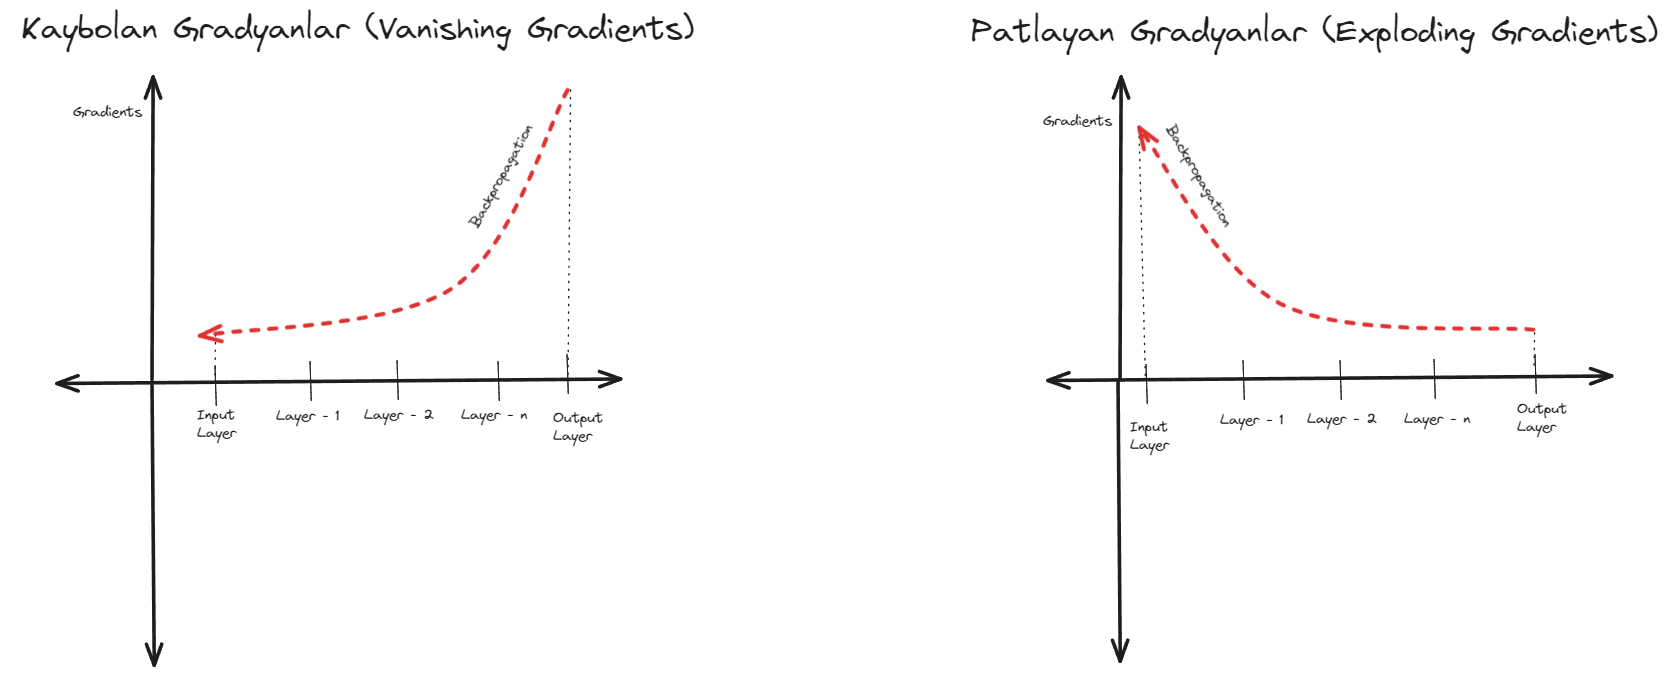
\includegraphics[width=1\textwidth]{images/gradient_problems.png}
    \caption{Gradyan problemleri.}
    \label{fig:enter-label}
\end{figure}

\subsection{Ortaya Çıkışı}
\begin{itemize}
    \item Sigmoid veya tanh gibi bazı aktivasyon fonksiyonları belirli aralılarda gradyanları küçültme eğilimindedir. Bu, geriye doğru gradyanların zamanla çok küçülmesine neden olabilir.
    \item Derin sinir ağları, birçok katmandan oluşur ve gradyanlar bu katmanlar arasında geriye doğru aktarılırken küçülebilir.
\end{itemize}

\subsection{Engelleme Yöntemleri}
\begin{itemize}
    \item ReLU, negatif girdiler için gradyanları sıfıra dönüştürmez, bu da gradyanların kaybolma riskini azaltır.
    \item Gradyanların belirli bir eşiğin altında veya üstünde tutulması, kaybolma riskini azaltabilir. Bu, gradyanların büyümesini kontrol eder ve daha dengeli bir eğitim süreci sağlar.
\end{itemize}

\newpage